\subsection{Experiment}

As a first method for proving our hypothesis we had to conduct a behavioral experiment in order to gather the data. We developed some basic user interface where an investment task was simulated.

The main idea of this experiment was to show to the people at each timestep either a price for which one of the houses in their neighborhood was sold or some belief of an "expert" (the Bayesian estimate based on the observation history) that shows the chances of the market being in a good state. Having this information, they had to decide when is the best moment to sell the house and maximize their profit. Together with this, after each timestept, the people were loosing a constant sum of money as a maintenance cost for keeping the house at that point.

You can see in ~\autoref{fig:user-interface} how the interface of the experiment looked like for the two main scenarios that we had: the observation experiment and the belief experiment. For the first scenario, at each timestep we show to the people a new observation together with all the past observations in  a plot, while for the second scenario we show them only the belief. Besides this, at all timesteps we also display the current maintenance cost that was lost until that point. 

\begin{figure}[!htbp]
    \centering
    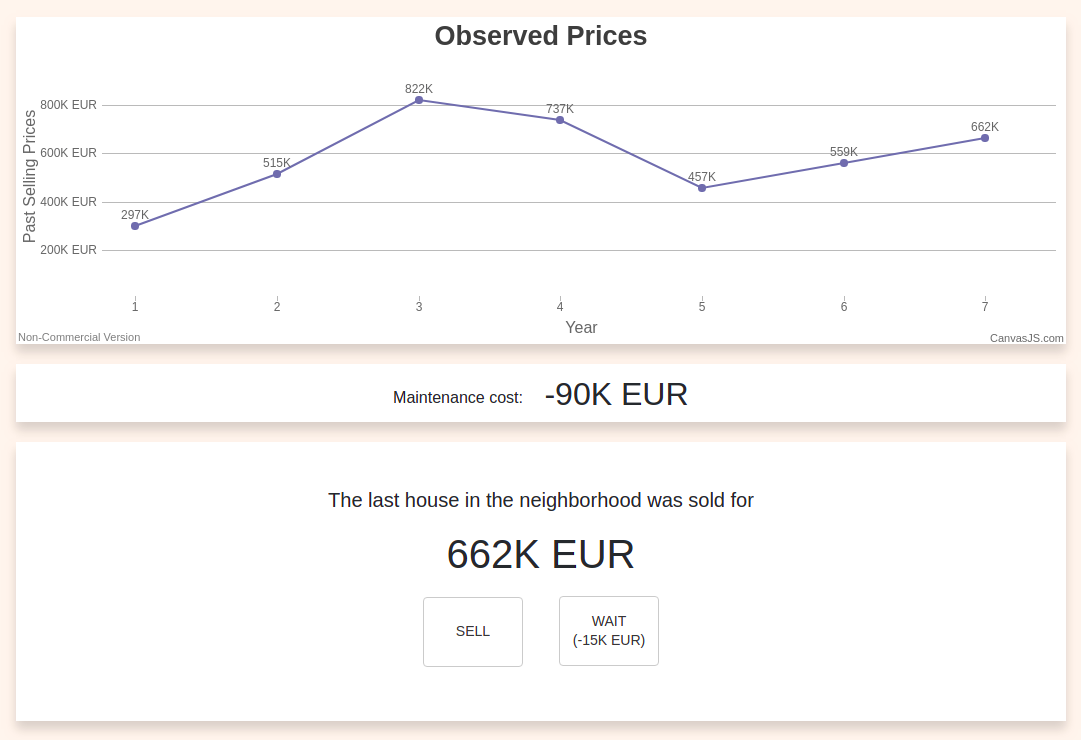
\includegraphics[width=0.99\linewidth]{img/methods/experiment_obs_1.png}\\
    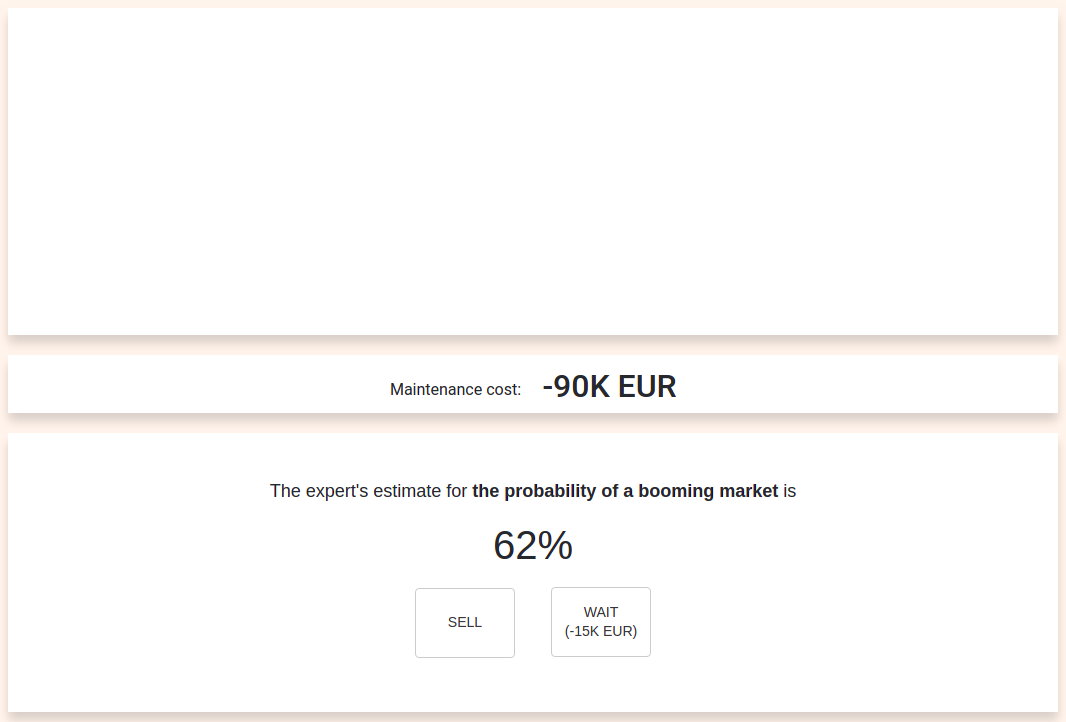
\includegraphics[width=0.99\linewidth]{img/methods/experiment_bel_1.png}\\
    \caption{The two experiment scenarios and their respective UI. In (a) subjects are shown the observation history at the top and a new observation at the bottom. In (b) they see the Bayesian estimate based on the observation history.}\label{fig:user-interface}
\end{figure}

In ~\autoref{fig:states} you can see a graphical representation of the expeeriment setup. The market has three states, \textit{recession} and \textit{booming} and \textit{sold}. The market starts in recession in each experiment and iteratively transitions are performed. At each transition subjects are shown an observation from the current state and can choose between \textit{wait} and \textit{sell}. The experiments ends when subjects sell and they receive a reward based on the last market state.

\begin{figure}[H]
\tikzset{
scale=0.62, every node/.append style={transform shape}
}
\begin {center}
\begin {tikzpicture}[-latex ,auto ,node distance =3cm and 4cm ,on grid ,
semithick , scale=0.5, transform shape,
state/.style ={ circle ,fill=black!20, minimum width =3 cm}]
\node[state] (C){$Sold$};
\node[state] (A) [above left=of C,align=center] {Recession};
\node[state] (B) [above right =of C,align=center] {Booming};
\coordinate[below of=A] (AA);
\coordinate[below of=B] (BB);
\coordinate[below of=AA] (D);
\coordinate[below of=BB] (E);

\path (A) edge [loop left, line width=1mm, align=center] node[left] {wait \\ $0.86$} (A);
\path (A) edge [bend left = -25,line width=1mm,align=center] node[below =0.25 cm] {sell\\$1.0$} (C);
\path (A) edge [bend left =25,line width=1mm,align=center] node[above] {wait\\$0.14$} (B);

\path (B) edge [loop right,line width=1mm,align=center] node[right] {wait\\$1.0$} (B);
\path (B) edge [bend right = -25,line width=1mm,align=center] node[below =0.25 cm] {sell\\$1.0$} (C);

%\fill[gray!40!white, opacity=0.5] (-6,-1) rectangle (5,6);

\path (A) edge [bend right =25,line width=1mm, dashed] node[left] {$Observation$} (D);
\path (B) edge [bend left  =25,line width=1mm, dashed] node[right] {$Observation$} (E);
\end{tikzpicture}
\end{center}
    \caption{Market States}\label{fig:states}
\end{figure}

In the end we run this experiment on 24 participants and each one of them did the following runs:
\begin{itemize}
    \item 20 runs with random samples from the observations experiment with an easy setup (low maintenance costs)
    \item 20 runs with random samples from the observations experiment with a hard setup (high maintenance costs)
    \item 50 runs with random samples from the belief experiment 
\end{itemize}

The participants were paid in the end according to their performance (average reward over all experiment runs) in order to give them some motivation for performing as good as possible in this experiment.

\subsection{Solving the risk sensitive POMDP}

\normalsize
Marecki \cite{marecki} showed that RSPOMDPs can be solved for arbitrary utility functions using \keyword{reverse value iteration} in Belief Wealth Space.
For this the original state space must be augmented two times:

\begin{figure}[H]
\begin {center}
\begin {tikzpicture}[-latex ,auto ,node distance =3cm and 3cm ,on grid,
semithick , state/.style ={ circle ,fill=black!20, maximum width =2 cm}]
\node[state] (A) [align=center] {Observation\\Time\\Space};
\node[state] (B) [right of=A,align=center] {Belief\\Time\\Space};
\node[state] (C) [right of=B,align=center] {Belief\\Wealth\\Space};

\path (A) edge [line width=1mm, align=center] node[left] {} (B);
\path (B) edge [line width=1mm,align=center] node[below =0.25 cm] {} (C);
\end{tikzpicture}
\end{center}
\end{figure}

First augmentation is done by describing the probability of being in the good state with a function $\phi(b,o)$ ~\autoref{m:belief-update}:

\begin{align}
    b' = \phi(b,o) := ()
\end{align}

This augmentation transforms the POMDP into a MDP.
Second augmentation ...